	\section{Динамика обилия {\it M.~balthica}.}

		\subsection{Эстуарий реки~Лувеньги.}


На литорали в эстуарии р.~Лувеньги средняя плотность поселений маком за период с $1992$ по $2012$ год колебалась от $55~(26,8)$ в $1992$ до $9200~(39,8)$~экз./м$^2$ в $1998$ году (рис. \ref{ris:dynamic_Kandalaksha_all}). 
	\begin{figure}[h]
	
	\begin{minipage}[b]{.46\linewidth}
	%Фигурка в первом ряду слева размер отведенный под весь этот объект \textendash 0.46 от ширины строки
	%Параметр [b] означает, что выравнивание этих министраниц будет по нижнему краю
	\begin{center}
	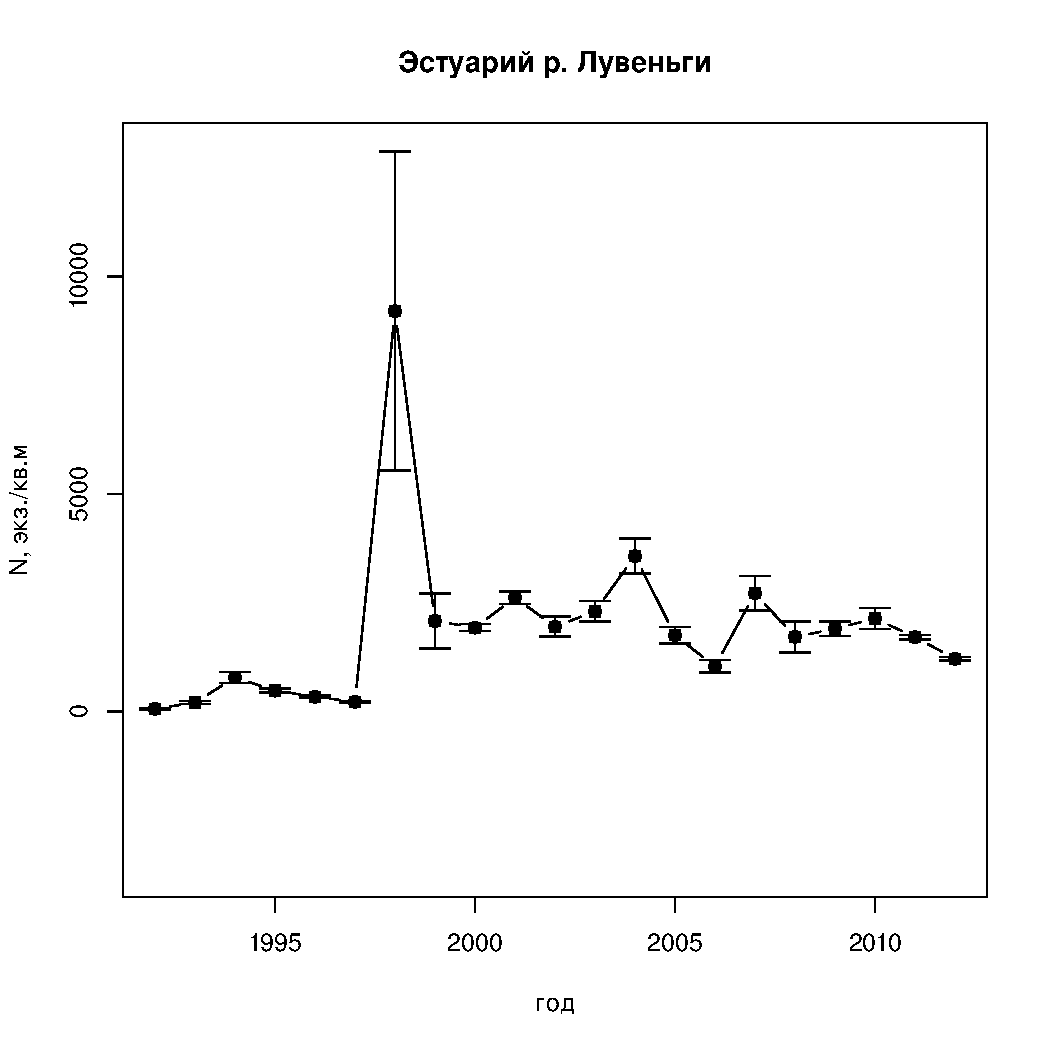
\includegraphics[width=65mm]{../White_Sea/Estuatiy_Luvenga/N_dynamic.pdf}

	\end{center}
	\end{minipage}
	%
	\hfil %Это пружинка отодвигающая рисунки друг от друга
	%
	\begin{minipage}[b]{.46\linewidth}
%Следующий рисунок - первый ряд справа %DUNGEON S_4 \ AB
	\begin{center}
		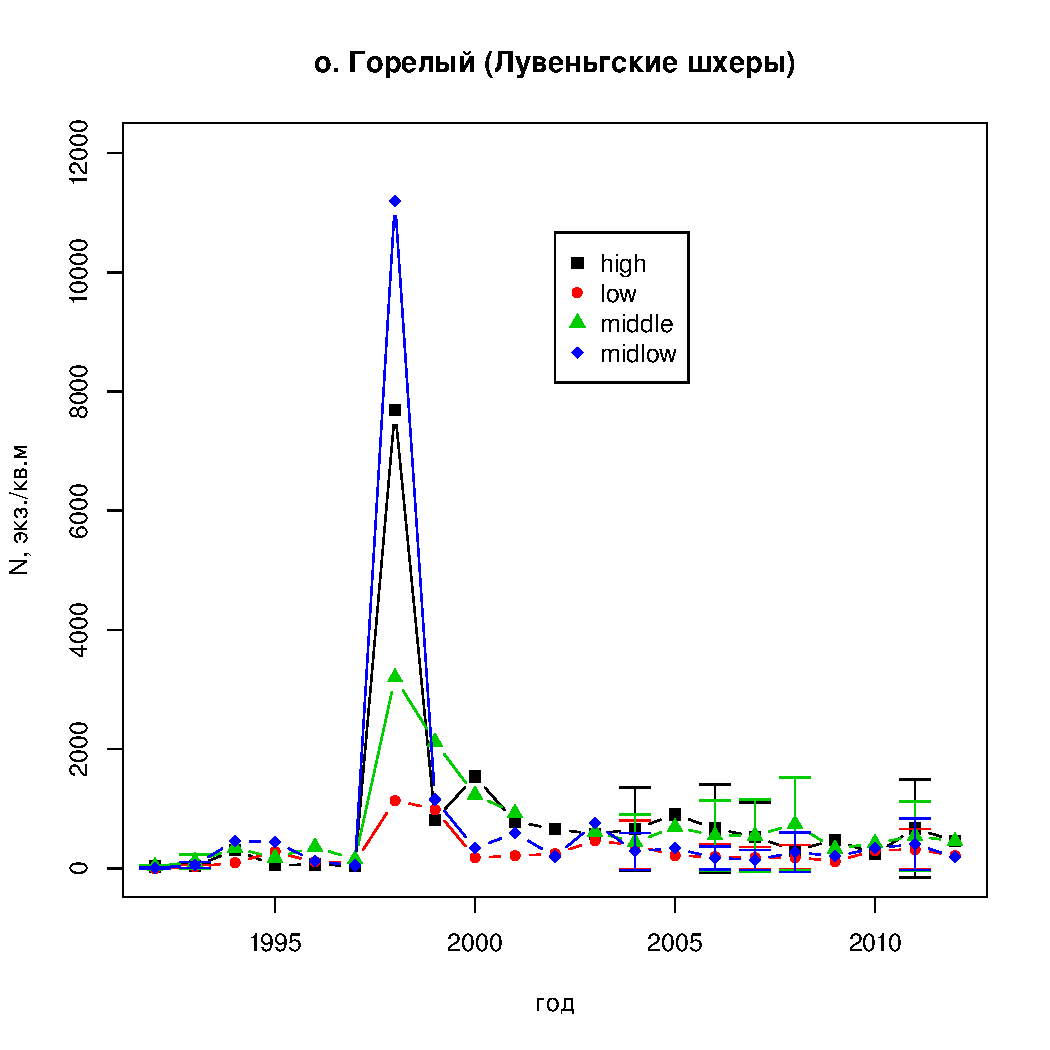
\includegraphics[width=65mm]{../White_Sea/Luvenga_Goreliy/N_dynamic.pdf}
	\end{center}
	\end{minipage}

%\smallskip


	\begin{minipage}[b]{.46\linewidth}
%Фигурка в первом ряду слева размер отведенный под весь этот объект \textendash 0.46 от ширины строки
%Параметр [b] означает, что выравнивание этих министраниц будет по нижнему краю
	\begin{center}
		\includegraphics[width=65mm]{../White_Sea//Luvenga_II_razrez/N_dynamic.pdf}
	\end{center}
	\end{minipage}
%
	\hfil %Это пружинка отодвигающая рисунки друг от друга
%
	\begin{minipage}[b]{.46\linewidth}
%Следующий рисунок - первый ряд справа %DUNGEON S_4 \ AB
	\begin{center}
		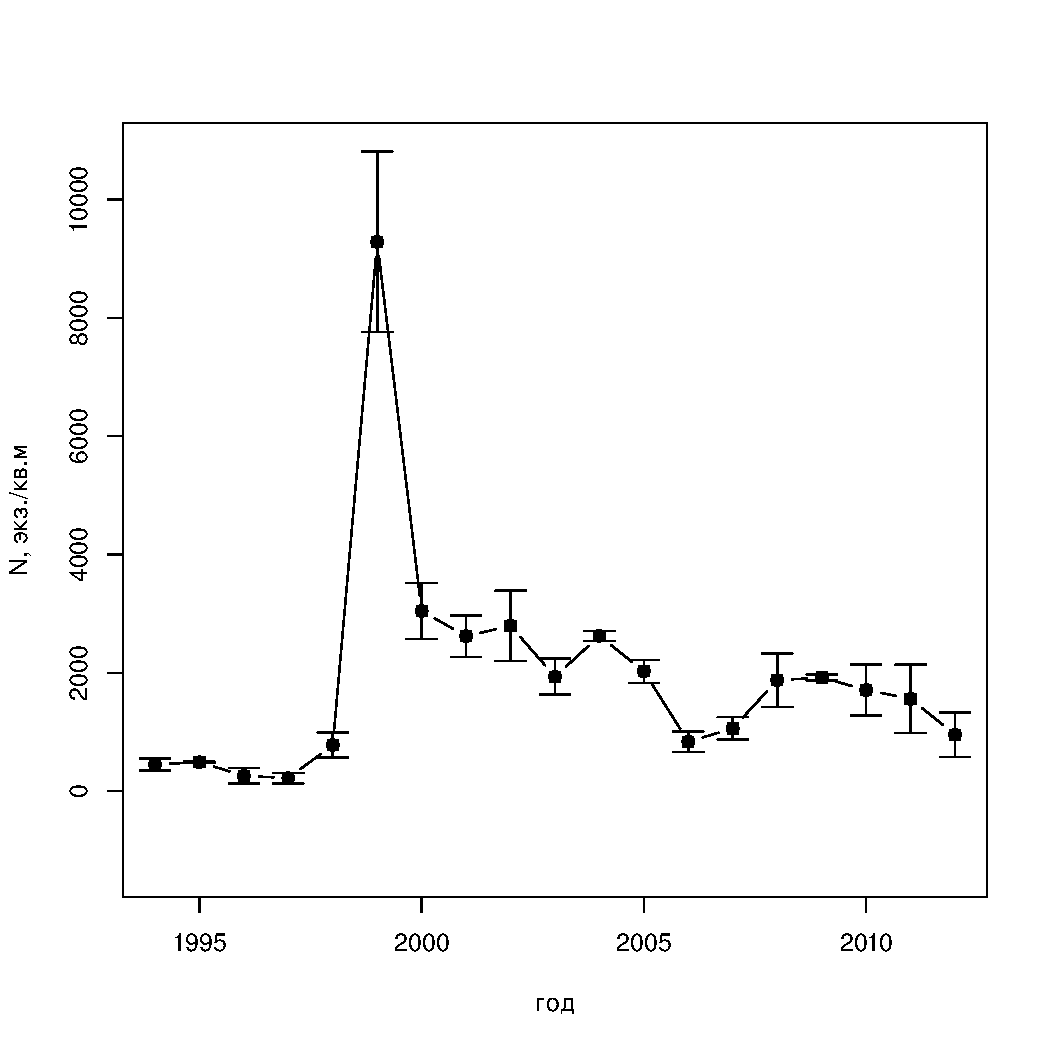
\includegraphics[width=65mm]{../White_Sea/Ryashkov_ZRS/N_dynamic.pdf}
	\end{center}
	\end{minipage}

%\smallskip

	\begin{minipage}[b]{.46\linewidth}
%Фигурка в первом ряду слева размер отведенный под весь этот объект \textendash 0.46 от ширины строки
%Параметр [b] означает, что выравнивание этих министраниц будет по нижнему краю
	\begin{center}
		\includegraphics[width=65mm]{../White_Sea/Ryashkov_YuG/N_dynamic.pdf}
	\end{center}
	\end{minipage}
%
	\hfil %Это пружинка отодвигающая рисунки друг от друга
%
	\begin{minipage}[b]{.46\linewidth}
%Следующий рисунок - первый ряд справа %DUNGEON S_4 \ AB
	\begin{center}
		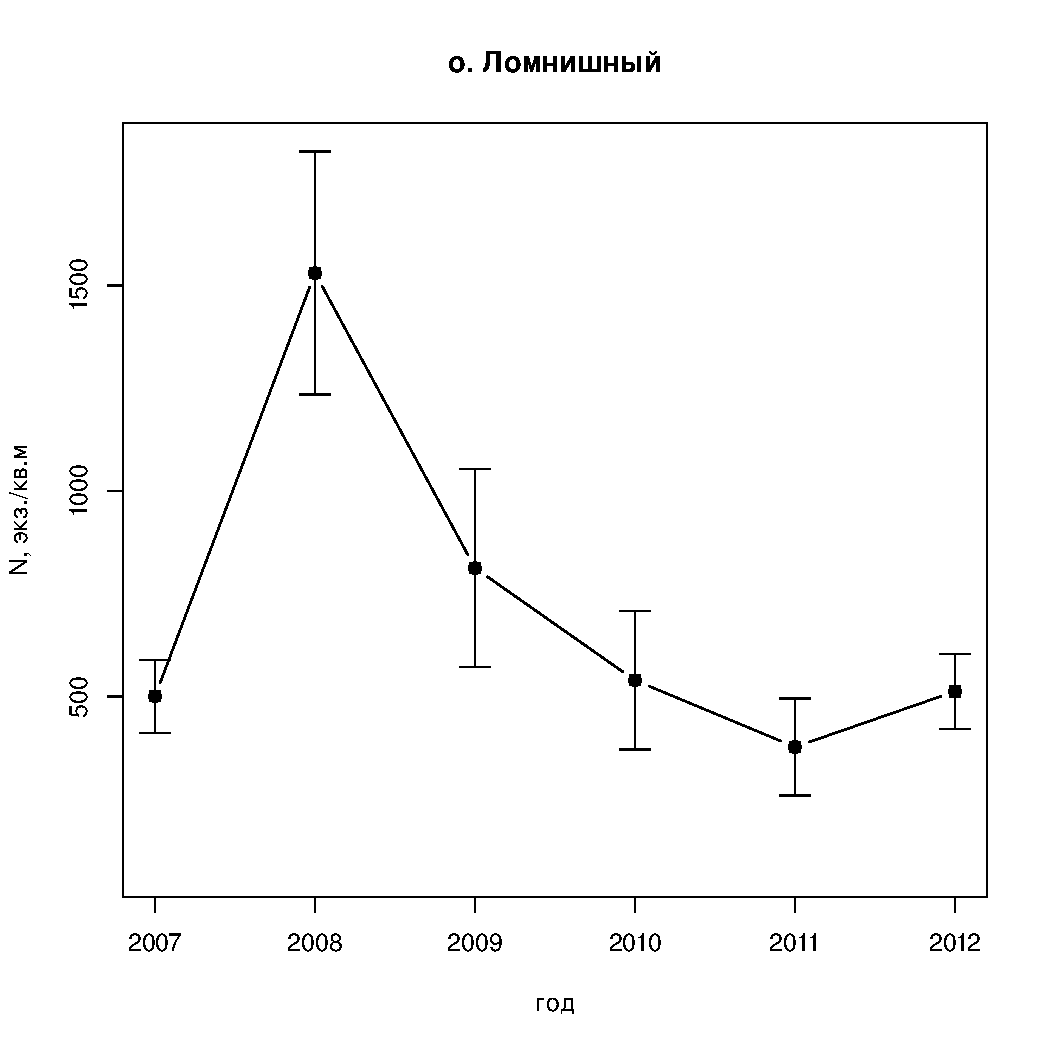
\includegraphics[width=65mm]{../White_Sea/Lomnishniy/N_dynamic.pdf}
	\end{center}
	\end{minipage}

%\smallskip


	\caption{Динамика плотности поселений {\it Macoma balthica} в вершине Кандалакшского залива}
	\label{ris:dynamic_Kandalaksha_all}
	\end{figure}
При этом столь высокая численность в $1998$ году была связана с особями длиной менее $1$~мм (рис. \ref{ris:dynamic_Kandalaksha_all2}) --- средняя численность моллюсков крупнее $1$~мм составляла всего $750~(2,03)$~экз./м$^2$.
	\begin{figure}[h]

	\begin{minipage}[b]{.46\linewidth}
%Фигурка в первом ряду слева размер отведенный под весь этот объект \textendash 0.46 от ширины строки
%Параметр [b] означает, что выравнивание этих министраниц будет по нижнему краю
	\begin{center}
		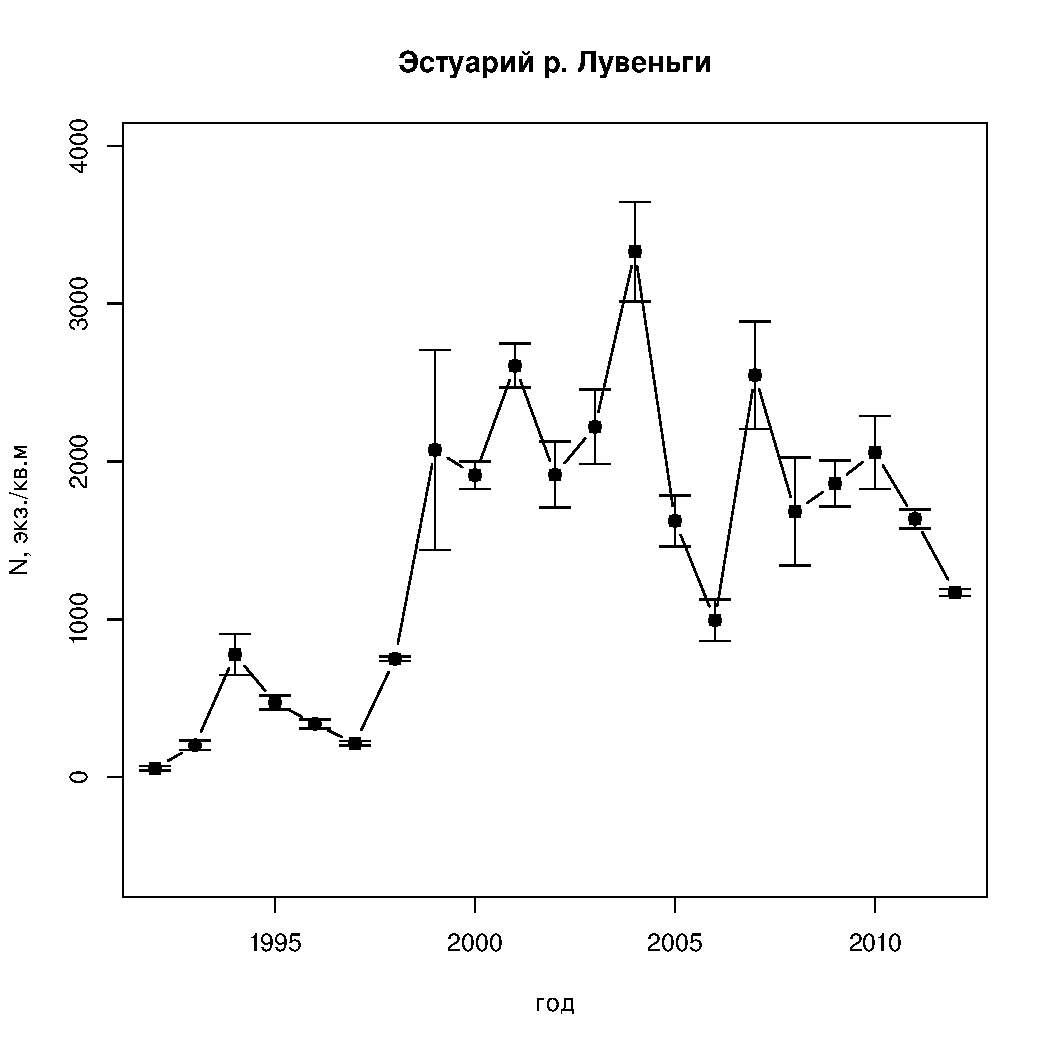
\includegraphics[width=65mm]{../White_Sea/Estuatiy_Luvenga/N2_dynamic.pdf}
	\end{center}
	\end{minipage}
%
	\hfil %Это пружинка отодвигающая рисунки друг от друга
%
	\begin{minipage}[b]{.46\linewidth}
%Следующий рисунок - первый ряд справа %DUNGEON S_4 \ AB
	\begin{center}
		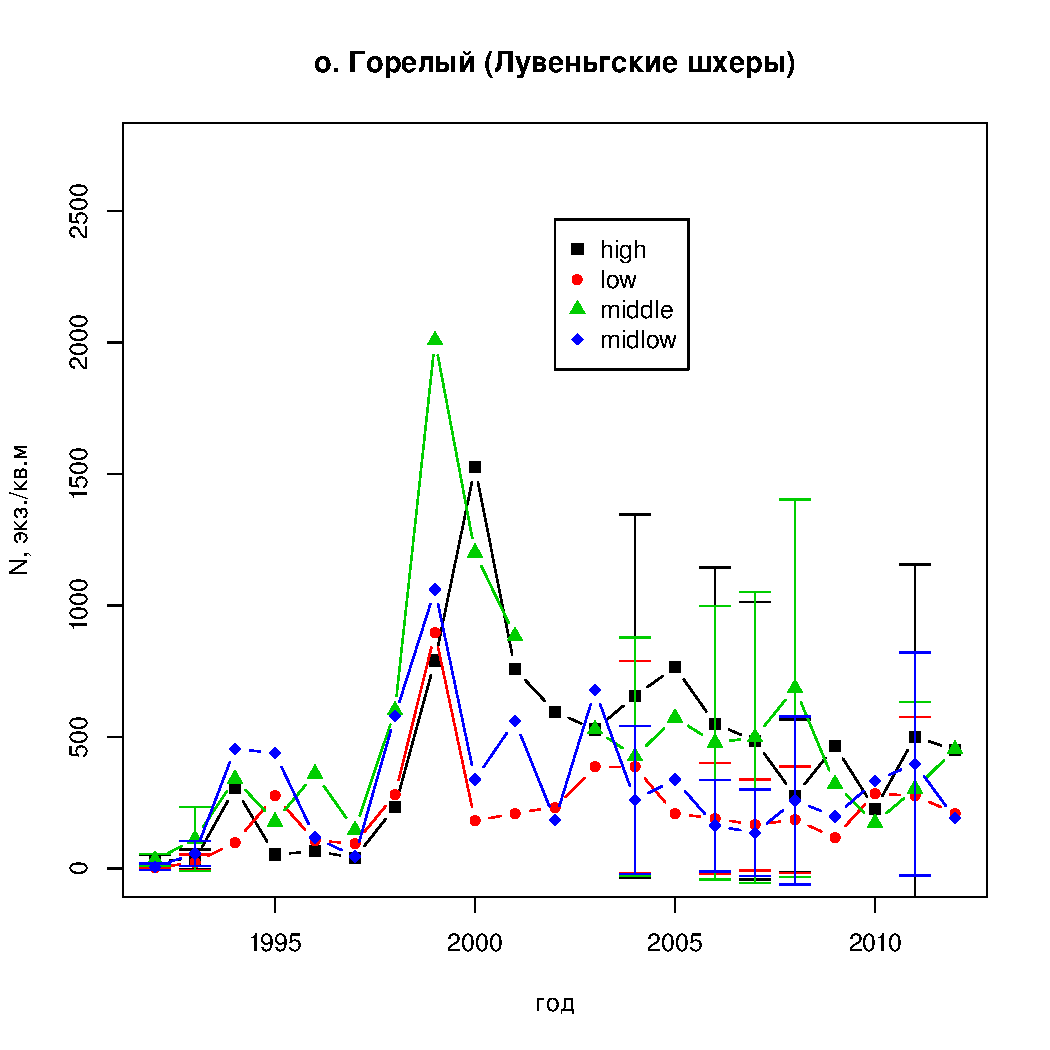
\includegraphics[width=65mm]{../White_Sea/Luvenga_Goreliy/N2_dynamic.pdf}
	\end{center}
	\end{minipage}
%\smallskip
	\begin{minipage}[b]{.46\linewidth}
%Фигурка в первом ряду слева размер отведенный под весь этот объект \textendash 0.46 от ширины строки
%Параметр [b] означает, что выравнивание этих министраниц будет по нижнему краю
	\begin{center}
		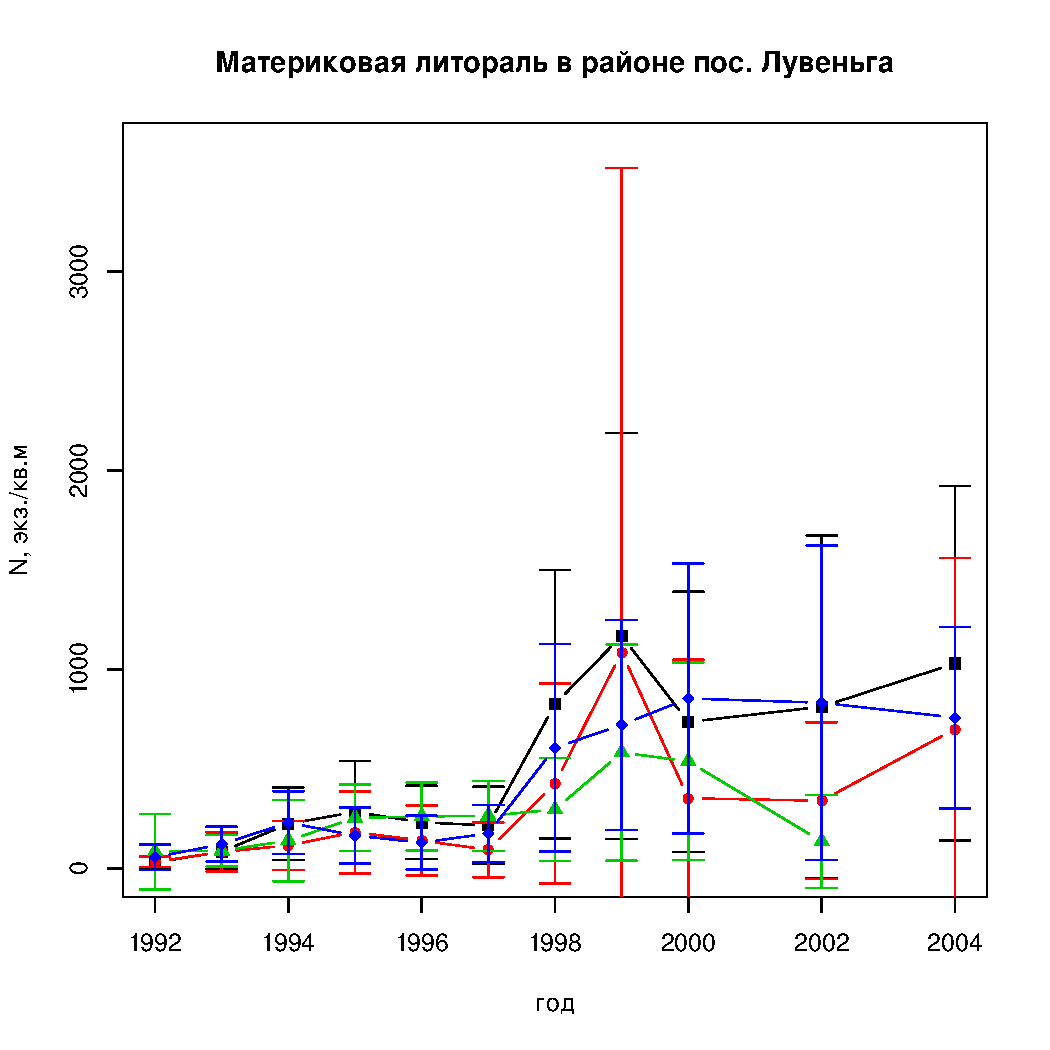
\includegraphics[width=65mm]{../White_Sea//Luvenga_II_razrez/N2_dynamic.pdf}
	\end{center}
	\end{minipage}
%
	\hfil %Это пружинка отодвигающая рисунки друг от друга
%
	\begin{minipage}[b]{.46\linewidth}
%Следующий рисунок - первый ряд справа %DUNGEON S_4 \ AB
	\begin{center}
		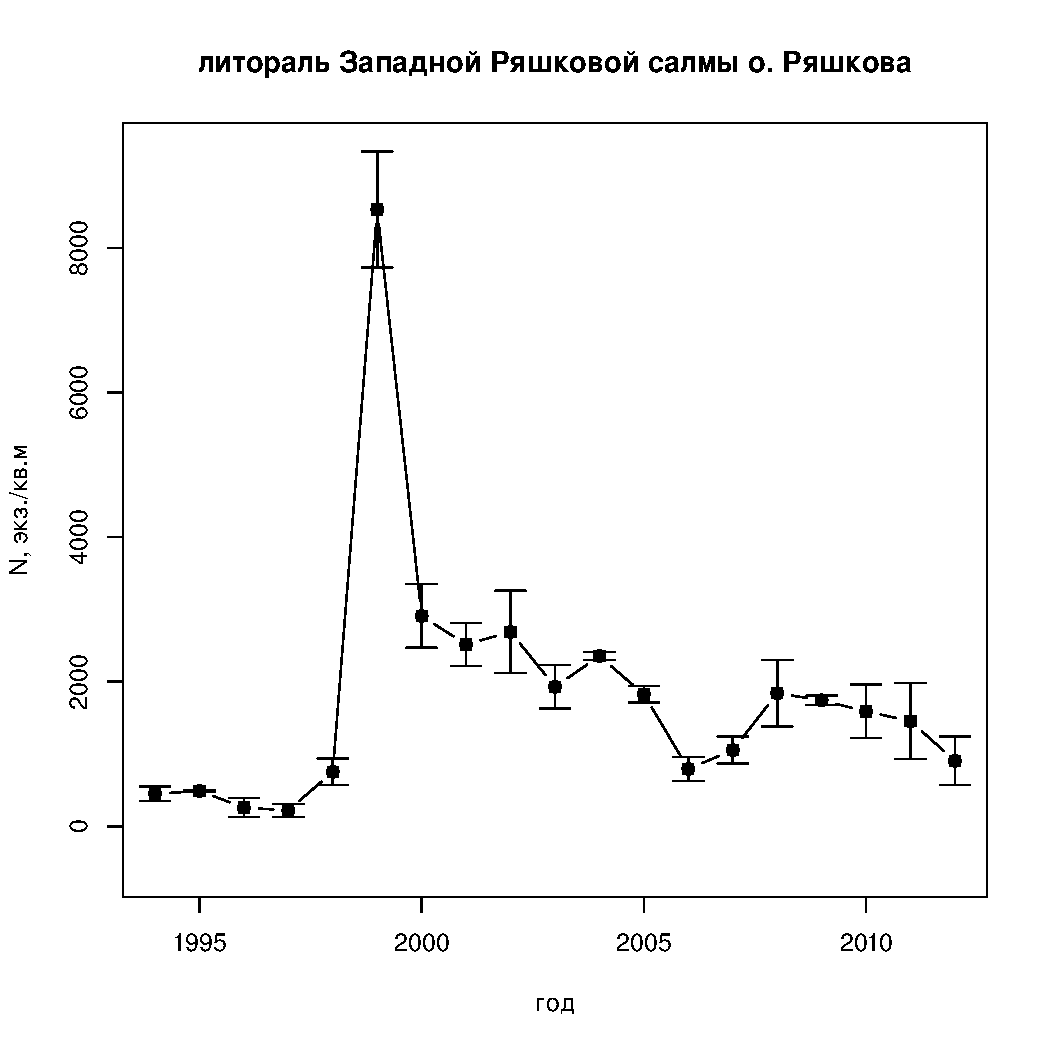
\includegraphics[width=65mm]{../White_Sea/Ryashkov_ZRS/N2_dynamic.pdf}
	\end{center}
	\end{minipage}
%\smallskip
	\begin{minipage}[b]{.46\linewidth}
%Фигурка в первом ряду слева размер отведенный под весь этот объект \textendash 0.46 от ширины строки
%Параметр [b] означает, что выравнивание этих министраниц будет по нижнему краю
	\begin{center}
		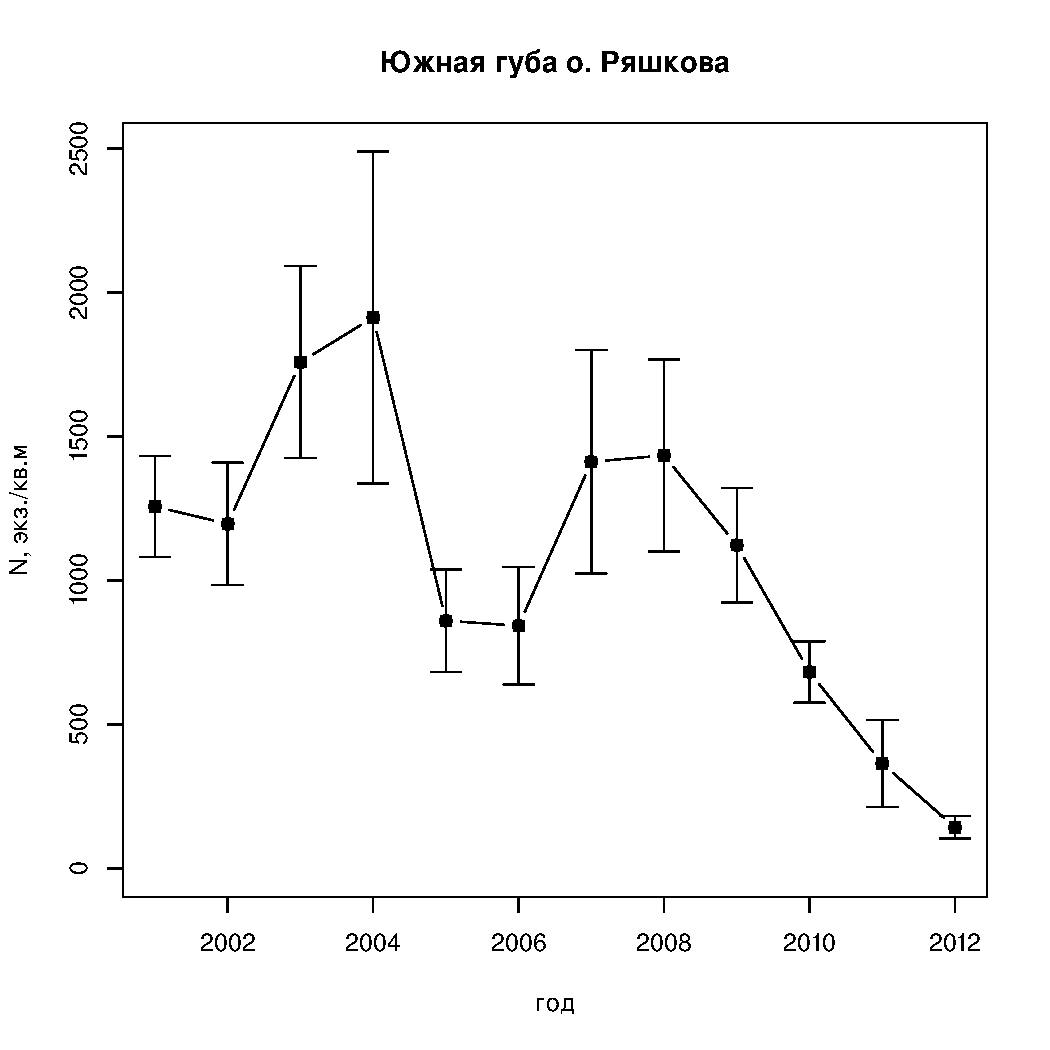
\includegraphics[width=65mm]{../White_Sea/Ryashkov_YuG/N2_dynamic.pdf}
	\end{center}
	\end{minipage}
%
	\hfil %Это пружинка отодвигающая рисунки друг от друга
%
	\begin{minipage}[b]{.46\linewidth}
%Следующий рисунок - первый ряд справа %DUNGEON S_4 \ AB
	\begin{center}
		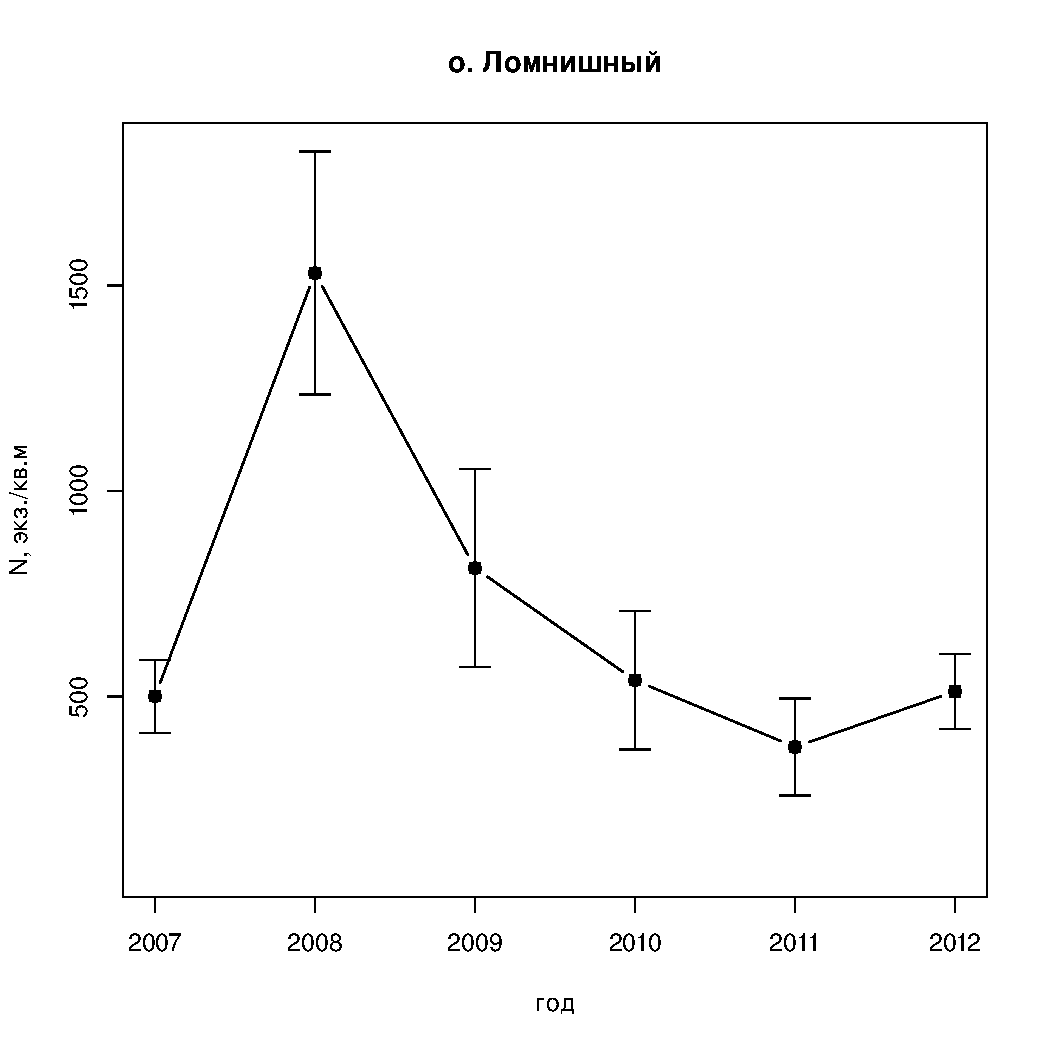
\includegraphics[width=65mm]{../White_Sea/Lomnishniy/N2_dynamic.pdf}
	\end{center}
	\end{minipage}

%\smallskip


	\caption{Динамика численности {\it Macoma balthica} с длиной раковины более $1$~мм в поселениях вершины Кандалакшского залива}
	\label{ris:dynamic_Kandalaksha_all2}
	\end{figure}



Для анализа динамики обилия, на наш взгляд, более информативно рассматривать численность без учета вновь осевших особей. 
\textcolor{red}{ОБЪЯСНЯТЬ ПРО ПОПОЛНЕНИЕ ПОСЕЛЕНИЯ ТУТ ИЛИ ГДЕ?}. 
Поскольку материал собирали в конце июля --- начале августа, то мы считаем спатом всех особей длиной менее $1$~мм. \textcolor{red}{сюда бы ссылку на размер спата в белом? Зубаха, Полоскин, Гольцев? Флячинская?} 
В этом случае можно говорить по крайней мере о двух периодах: с $1992$ по $1998$ год --- период относительно низкой численности (менее $800$~экз./м$^2$ ) моллюсков, и с $1999$ по $2012$ год --- относительно высокой (более $1000$~экз./м$^2$) (достоверные различия по критерию Манна-Уитни, $W = 6, p-value = 4,5 \times 10^{-13}$) (рис.~\ref{ris:dynamic_Kandalaksha_all2}).

В период с $1992$ по $1998$ год численность {\it M.~balthica} достоверно изменялась ($Kruskal-Wallis\ \chi^2 = 24,1, p-value = 0,00049$). Результаты попарного сравнения представлены в таблице \ref{tab:Tukey_estuary_92_98_n2}.

	\begin{table}
	\begin{tabular}{|*{4}{p{0.2\textwidth}|}} \hline
	годы & различия средних & p-value & достоверность различий\\
	\hline
	$1993-1992$ & $147$ &  $0,11$ & \\
	\hline
	$1994-1993$ & $575$  & $2,47 \times 10^{-7}$ & *** \\
	\hline
	$1995-1994$ & $-303$  & $0,0069$ & ** \\
	\hline
	$1996-1995$ & $-137$  & $0,51$ & \\
	\hline
	$1997-1996$ & $-123$  & $0,62$ & \\
	\hline
	$1998-1997$ & $537$  & $6,73 \times 10^{-6}$ & *** \\
	\hline
	\end{tabular}

	{\footnotesize Примечание: достоверность различий *** --- $p<0,001$; ** --- $p<0,05$; * --- $p<0,1$.}
	\caption{Результаты множественного сравнения средних численностей {\it Macoma balthica} методом Тьюки (Tukey's ‘Honest Significant Difference’) в эстуарии реки Лувеньги в $1992-1998$ годах.}
	\label{tab:Tukey_estuary_92_98_n2}
	\end{table}

Численность моллюсков в эстуарии р. Лувеньги в $1992-1993$ годах оставалась стабильной ($\bar{N} = 128~(21,5)$~экз./м$^2$), затем произошло ее увеличение в $1994$ году, после чего снова произошло некоторое ее снижение и в $1995 - 1997$ годах она стабилизировалась на более высоком уровне ($\bar{N} = 341~(9,3)$~экз./м$^2$) по сравнению с $1992 - 93$ гг.
В $1998$ году вновь происходит увеличение численности {\it M.~balthica} до уровня $1994$ года (около $750 - 800$~экз./м$^2$), после чего в $1999$ году средняя численность возросла ещё в три раза.
С $1999$ по $2003$ год численность оставалась относительно стабильной  ($Kruskal-Wallis\ \chi^2 = 5,0, p-value = 0,28$) и в среднем составляла $2146~(5,5)$~экз./м$^2$.
В $2004$ году обилие маком увеличилось в полтора раза и достигло максимума для данного участка за весь период наблюдений. 
С $2004$ по $2006$ год численность моллюсков последовательно снижалась (табл.~\ref {tab:Tukey_estuary_04_07_n2}). 
	\begin{table}
	\begin{tabular}{|*{4}{p{0.2\textwidth}|}} \hline
	годы & различия средних & p-value & достоверность различий\\
	\hline
	$2005-2004$ & $-1707$ & $0,09$ & *\\
	\hline
	$2006-2005$ & $-630$ & $0,78$ & \\
	\hline
	$2007-2006$ & $1553$ & $0,05$ & **\\
	\hline
	\end{tabular}

	{\footnotesize Примечание: достоверность различий *** --- $p<0,001$; ** --- $p<0,05$; * --- $p<0,1$.}
	\caption{Результаты множественного сравнения средних численностей {\it Macoma balthica} методом Тьюки (Tukey's ‘Honest Significant Difference’) в эстуарии реки Лувеньги в $2004-2007$ годах.}
	\label{tab:Tukey_estuary_04_07_n2}
	\end{table}
В $2006$ году она достигла локального минимума и составляла $993~(13,2)$~экз./м$^2$). 
В $2007$ году произошло достоверное увеличение численности {\it Macoma balthica} (табл.~\ref {tab:Tukey_estuary_04_07_n2}).
К $2008$ году численность моллюсков снова снижается, после чего до $2012$ года были отмечены недостоверные флуктуации ($Kruskal-Wallis\ \chi^2 = 6,8429, p-value = 0,14$).

		\subsection{Илистая губа острова Горелый.}
\textcolor{red}{посчитать и вписать относительные ошибки}
На данном участке рассматривали отдельно 4 зоны, различающиеся по осушке и биотическим условиям. 
Максимальная численность маком на всех горизонтах литорали была отмечена в $1998$ году (рис.~\ref{ris:dynamic_Kandalaksha_all}).
Более чем на 75\% такая высокая численность была связана с обилием особей длиной менее $1$~мм.
Максимальная численность моллюсков наблюдалась на границе среднего и нижнего горизонта в зарослях фукоидов, здесь она составляла более $44$~тысяч~экз./м$^2$.

При исключении из анализа особей размером менее $1$~мм, численность особей {\it M.~balthica} стала максимальной в $1999$ году для всех горизонтов, кроме среднего, на котором максимальная численность отмечена в $2000$ году (рис.~\ref{ris:dynamic_Kandalaksha_all2}).
Самая низкая чиленность за весь период исследований была отмечена в начале интервала наблюдений ($1992-1993$~года) --- менее $100$~экз./м$^2$.
С $1994$ по $1996$~год происходило некоторое увеличение численности маком, однако она на всех горизонтах не превышала $500$~экз./м$^2$.
В $1997$ году произошло локальное снижение численности, и c $1998$~года происходил ее рост. 
В $1999$ году численность маком составляла $900$, $2000$ и $1050$~экз./м$^2$ на среднем горизонте, в поясе фукоидов и у нуля глубин, соответсвенно.
В $2000$ году на верхнем горизонте литорали численность особей достиглаа максимума за весь период наблюдений и составила  $1500$~экз./м$^2$, в то время как на остальных горизонтах литорали произошло снижение численности.
В дальнейшем были отмечены менее значительные колебания, и, как показывают данные в $2004$, $2006 - 2008$ и $2011$ годах (когда на станциях брали индивидуальные пробы, а не интегрированные) эти колебания недостоверны (табл.~\ref{tab:Goreliy_N2_Kruskal}).

	\begin{table}
	\begin{tabular}{|*{4}{p{0.25\textwidth}|}} \hline
	горизонт литорали & $Kruskal-Wallis\ \chi^2$ & $p-value$ & $\bar{N} ~ (D)$ \\ 
	\hline
	верхний & $0,91$ & $0,92$ & $1972~(11,4)$ \\
	\hline
	средний & $1,37$ & $0,85$ & $1910~(9,0)$\\
	\hline
	пояс фукоидов & $2,13$ & $0,71$ & $970~(13,7)$ \\
	\hline
	нижний & $3,45$ & $0,49$ & $960~(10,6)$ \\
	\hline
	\end{tabular}
	{\footnotesize Примечание: Kruskal-Wallis $\chi^2$ --- значения критерия Краскелл-Уоллиса; $\bar{N}$ --- средняя численность {\it 	M.~balthica}, экз./м$^2$; $D$ --- относительная ошибка средней, \%.}
	\caption{Межгодовое различие численности {\it Macoma~balthica} на литорали о.~Горелый по данным $2004$, $2006 - 2008$ и $2011$ годов.}
	\label{tab:Goreliy_N2_Kruskal}
	\end{table}


		\subsection{Материковая литораль в районе пос. Лувеньга}

На материковой литорали в районе поселка Лувеньга отдельно рассматривали динамику поселений {\it M.~balthica} в четырех зонах, отличающихся по осушке и биотическим условиям.
За весь период наблюдений максимальные флуктуации численности маком были отмечены для зоны верхнего пляжа: от $94~(38~\%)$~экз./м$^2$ в $1992$ до $16365~(53~\%)$~экз./м$^2$ в $1998$ году (\ref{ris:dynamic_Kandalaksha_all}). 
Доля спата в большинстве выборок составляет менее $20~\%$, исключение составляет зона верхнего пляжа в $1998$, где доля спата была $87~\%$.
В дальнейшем мы рассматриваем динамику обилия без учета спата (рис.~\ref{ris:dynamic_Kandalaksha_all2}).

В начале периода наблюдения численность на всех трех участках не превышала $1000$~экз./м$^2$ и колебания носили случайный характер (табл.~\ref{tab:2razrez_N2_Kruskal}).

	\begin{table}
	\begin{tabular}{|*{4}{p{0.25\textwidth}|}} \hline
	зона & $Kruskal-Wallis\ \chi^2$ & $p-value$ & $\bar{N} ~ (D)$ \\ 
	\hline
	верхний пляж & $3,57$ & $0,61$ & $477~(16,6)$ \\
	\hline
	пояс фукоидов & $12,8$ & $0,02$ & $ $\\
	\hline
	пояс зостеры & $2,13$ & $0,71$ & $970~(13,7)$ \\
	\hline
	нижний пляж & $3,45$ & $0,49$ & $960~(10,6)$ \\
	\hline
	\end{tabular}
	{\footnotesize Примечание: Kruskal-Wallis $\chi^2$ --- значения критерия Краскелл-Уоллиса; $\bar{N}$ --- средняя численность {\it 	M.~balthica}, экз./м$^2$; $D$ --- относительная ошибка средней, \%.}
	\caption{Межгодовое различие численности {\it Macoma~balthica} на материковой литорали в районе поселка Лувеньга с $1992$ по $1998$ год.}
	\label{tab:2razrez_N2_Kruskal}
	\end{table}


		\subsection{Литораль Западной Ряшковой салмы о.~Ряшкова.}

На данном участке литорали средняя плотность поселений {\it M.~balthica} за период с $1994$ по $2012$ год колебалась от $220~(40,9)$~экз./м$^2$ в $1997$ до $9285~(16,4)$~экз./м$^2$ в $1999$~году (рис. \ref{ris:dynamic_Kandalaksha_all}).
При исключение из рассмотрения особей длиной менее $1$~мм минимальная средняя численность не изменилась, а максимальная в $1999$ составила $8530~(9,4)$~экз./м$^2$ (рис. \ref{ris:dynamic_Kandalaksha_all2}).
Однако столь высокая численность не сохранилась дольше одного года, и в период с $2000$ по $2012$ колебалась в пределах $1 \textendash 2,5$~тысяч~экз./м$^2$, в среднем составляя $1823~(8,0)$~экз./м$^2$.
Тем не менее, после $1999$ года средняя численность маком достоверно больше ($W = 4,5, p-value = 1,007 \times 10^{-5}$), чем до --- $2145~(4,5)$ и $435~(17,2)$, соответственно.

Минимальная численность в период после $2000$~года была отмечена в 2006 году и составляла $795~(20,8)$~экз./м$^2$. 
Периоды с $2000$ по $2006$ и с $2007$ по $2012$ годы достоверно различаются ($W = 131,5, p-value = 0,016$) по средней численности маком ($2146~(9,5)$ и $1448~(10,8)$, соответственно).

Внутри каждого периода времени численность {\it M.~balthica} не различается достоверно от года к году (табл. \ref{tab:ZRS_N2_Kruskal}).

	\begin{table}
	\begin{tabular}{|*{4}{p{0.25\textwidth}|}} \hline
	годы наблюдения & $Kruskal-Wallis\ \chi^2$ & $p-value$ & $\bar{N} ~ (D)$ \\ 
	\hline
	$1994 - 1998$ & $7,2$ & $0,12$ & $435~(17,2)$ \\
	\hline
	$2000 - 2006$ & $9,8$ & $0,13$ & $2146~(9,5)$\\
	\hline
	$2007 - 2012$ & $4,9$ & $0,43$ & $1448~(10,8)$ \\
	\hline
	\end{tabular}
	{\footnotesize Примечание: Kruskal-Wallis $\chi^2$ --- значения критерия Краскелл-Уоллиса; $\bar{N}$ --- средняя численность {\it 	M.~balthica}, экз./м$^2$; $D$ --- относительная ошибка средней, \%.}
	\caption{Межгодовое различие численности {\it Macoma~balthica} на литорали Западной Ряшковой салмы о.~Ряшкова в разные годы.}
	\label{tab:ZRS_N2_Kruskal}
	\end{table}


		\subsection{Южная губа острова Ряшкова}
Поскольку на литорали Южной губы о.~Ряшкова использовали для промывки сито с диаметром ячеи $1$~мм, то доля моллюсков размером менее $1$~мм не превышала $1,2~\%$ и их исключение из анализа не изменило общей картины.
На данном участке с $2001$ по $2010$ год численность {\it Macoma~balthica} была относительно стабильна, все флуктуации были недостоверны ($Kruskal-Wallis\ \chi^2 = 12,07, p-value = 0,21$). 
Средняя численность за данный период составила $1239~(7,9)$~экз./м$^2$.
Однако намечается некоторая тенденция к увеличению численности в $2003-2004$ и $2007-2008$ году.
После $2008$ года численность постепенно снижается и в $2012$ году она составила $142~(27,5)$~экз./м$^2$.

		\subsection{Остров Ломнишный}
На литорали о.~Ломнишный для промывки также использовали сито с диаметром ячеи $1$~мм, моллюски длиной менее 1 мм в пробах отсутствовали.
На данном участке численность маком оставалась относительно стабильной в течении всего периода исследований ($Kruskal-Wallis\ \chi^2 = 9,9, p-value = 0,077$) и в среднем составляла $638~(12)$~экз./м$^2$.
Некоторое увеличение численности было отмечено в $2008$ году (численность составляла $1530~(19)$~экз./м$^2$).


	\subsection{Анализ динамики численности {\it Macoma balthica} в Кандалакшском заливе Белого моря}
При изучении динамики численности можно анализировать несколько компонентов.
Первый компонент --- наличие или отсутсвие тренда как направленноого изменения численности.
При убирании тренда остается компонент динамики, для которого двумя крайими случаями будет: стабильная численность, которая поддерживается за счет плотностнозависимых процессов как систем обраной связи и неконтролируемый рост численности популяции по экспоненте.

Мы проанализировали динамику численности {\it M.~balthica} на каждом участке на наличие тренда при помощи теста Мантеля (табл.~\ref{tab:Mantel_N2_trend}).
	\begin{table}[ht]
	\caption{Выявление трендов в динамике численности {\it Macoma balthica} на различных участках Белого моря.}
	\label{tab:Mantel_N2_trend}
        \begin{tabular}{|p{0.25\textwidth}|*{2}{p{0.2\textwidth}|p{0.25\textwidth}|}} \hline
	Участок & $Mantel$ & $p$ & наличие тренда
	\\ \hline
	Эстуарий р. Лувеньга & 0,3168 & 0,003 & есть
	\\ \hline
	о. Горелый & 0,0269 & 0,368 & нет
	\\ \hline
	материковая литораль (Лувеньга) & 0,6103 & 0,001 & есть
	\\ \hline
	Южная губа о. Ряшков & 0,3687 & 0,015 & есть
	\\ \hline
	Запдная Ряшкова салма & 0,0108 & 0,404 & нет
	\\ \hline
	Ломнишный & -0,0999 & 0,47 & нет
	\\ \hline
	г. Медвежья & 0,0154 & 0,385 & нет
	\\ \hline
	г. Сельдяная & 0,2524 & 0,003 & есть
	\\ \hline
	\end{tabular}
	%    {\footnotesize Примечание: достоверность различий *** \textemdash $p<0,001$; ** \textemdash $p<0,05$; * \textemdash $p<0,1$.}
	\end{table}

Было показано наличие тренда на 4 участках: эстуарий р.~Лувеньга, материковая литораль в районе пос. Лувеньга, Южная губа о.~Ряшкова, г. Сельдяная.
Для удаления тренда из исходных значений были вычтены предсказанные значения из регрессионной модели $N = a + b*T$, где $N$ --- численность, экз./м$^2$, $T$ --- годы.
По детрендированному ряду были рассчитаны частные автокорреляции ($PRCF$ - partial rate correlation function).  
Коррелограммы представлены на рисунке \ref{ris:perm_PRCF_Kandalaksha_N2_detrend}.
	\begin{figure}[ht]
	
	\begin{minipage}[b]{.46\linewidth}
	%Фигурка в первом ряду слева размер отведенный под весь этот объект \textendash 0.46 от ширины строки
	%Параметр [b] означает, что выравнивание этих министраниц будет по нижнему краю
	\begin{center}
	{\footnotesize Эстуарий р.~Лувеньги}
		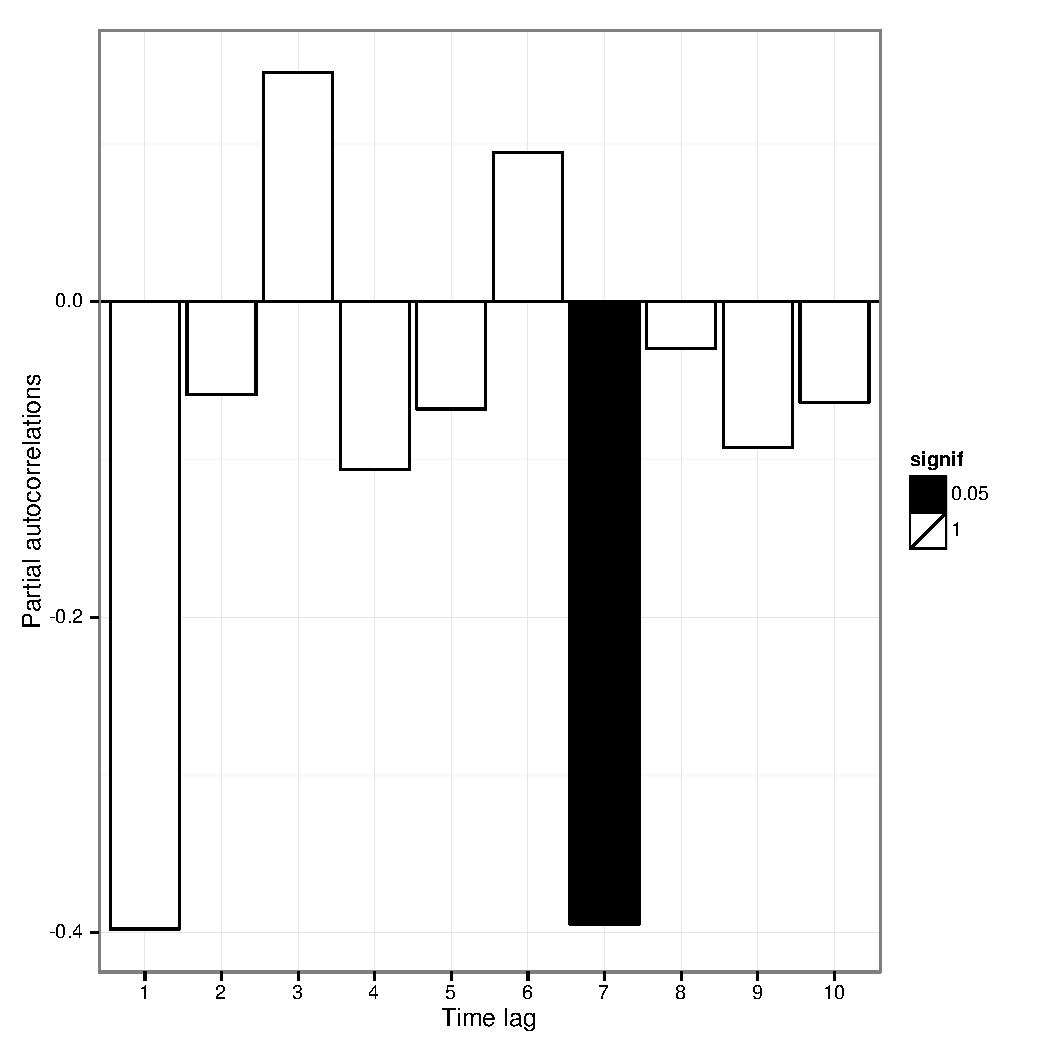
\includegraphics[width=65mm]{../White_Sea/dynamic_N_N1/perm_PRCF_Estuary_detrend.pdf}

	\end{center}
	\end{minipage}
		\hfil %Это пружинка отодвигающая рисунки друг от друга
	\begin{minipage}[b]{.46\linewidth}
%Следующий рисунок - первый ряд справа %DUNGEON S_4 \ AB
	\begin{center}
	{\footnotesize о.~Горелый}
		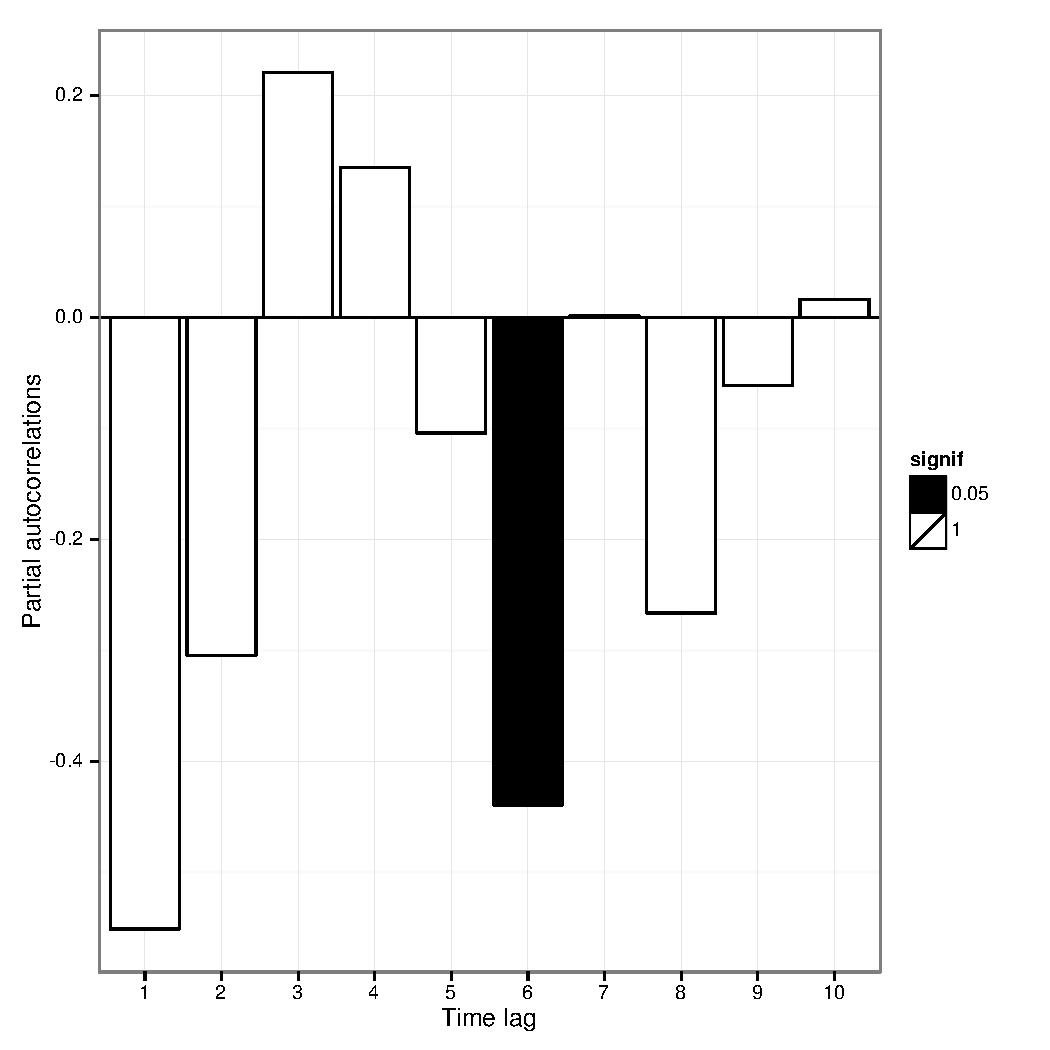
\includegraphics[width=65mm]{../White_Sea/dynamic_N_N1/perm_PRCF_Goreliy_all_detrend.pdf}
	\end{center}
	\end{minipage}

	\begin{minipage}[b]{.46\linewidth}
%Фигурка в первом ряду слева размер отведенный под весь этот объект \textendash 0.46 от ширины строки
%Параметр [b] означает, что выравнивание этих министраниц будет по нижнему краю
	\begin{center}
	{\footnotesize материковая литораль (Лувеньга)}
	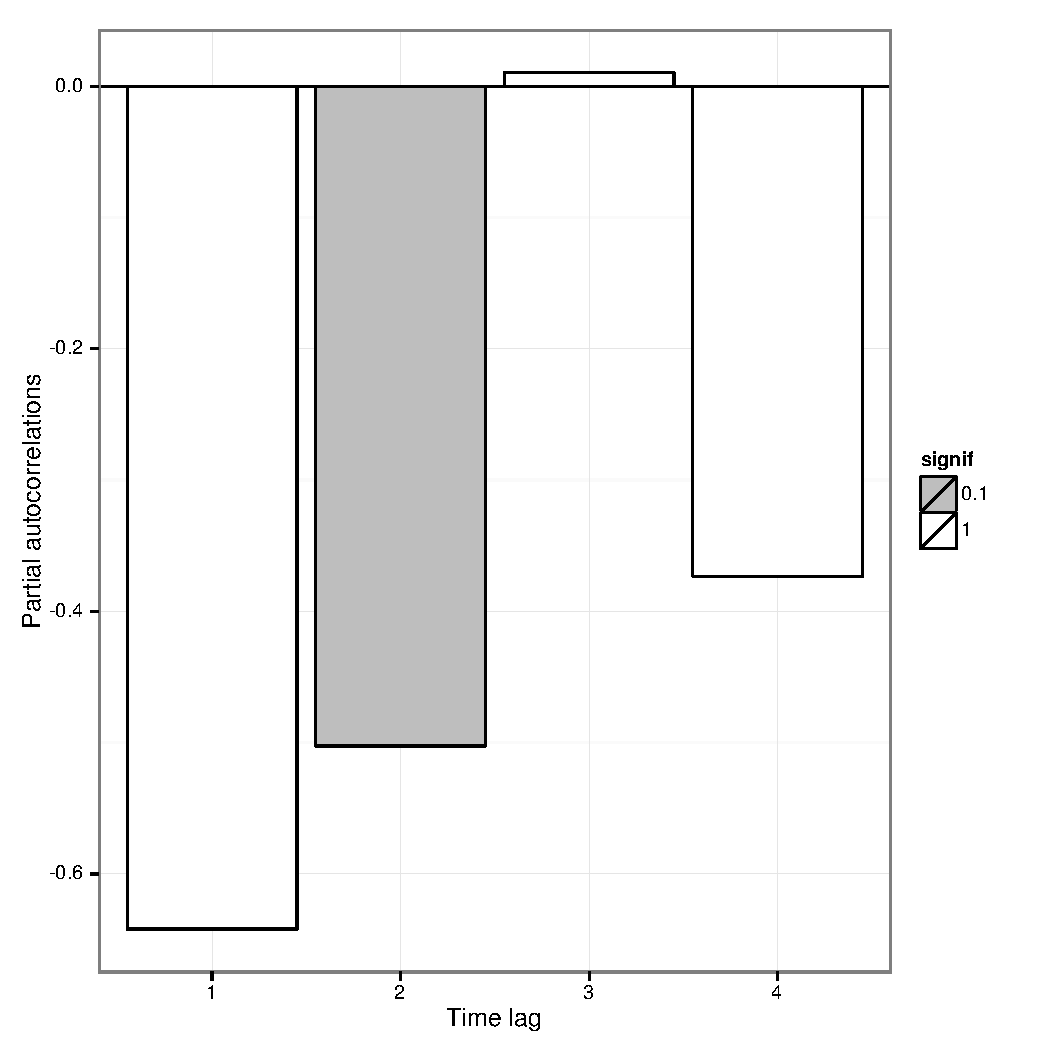
\includegraphics[width=65mm]{../White_Sea/dynamic_N_N1/perm_PRCF_razrez2_all_detrend.pdf}
	\end{center}
	\end{minipage}
		\hfil %Это пружинка отодвигающая рисунки друг от друга
	\begin{minipage}[b]{.46\linewidth}
%Следующий рисунок - первый ряд справа %DUNGEON S_4 \ AB
	\begin{center}
	{\footnotesize о.~Ломнишный}
	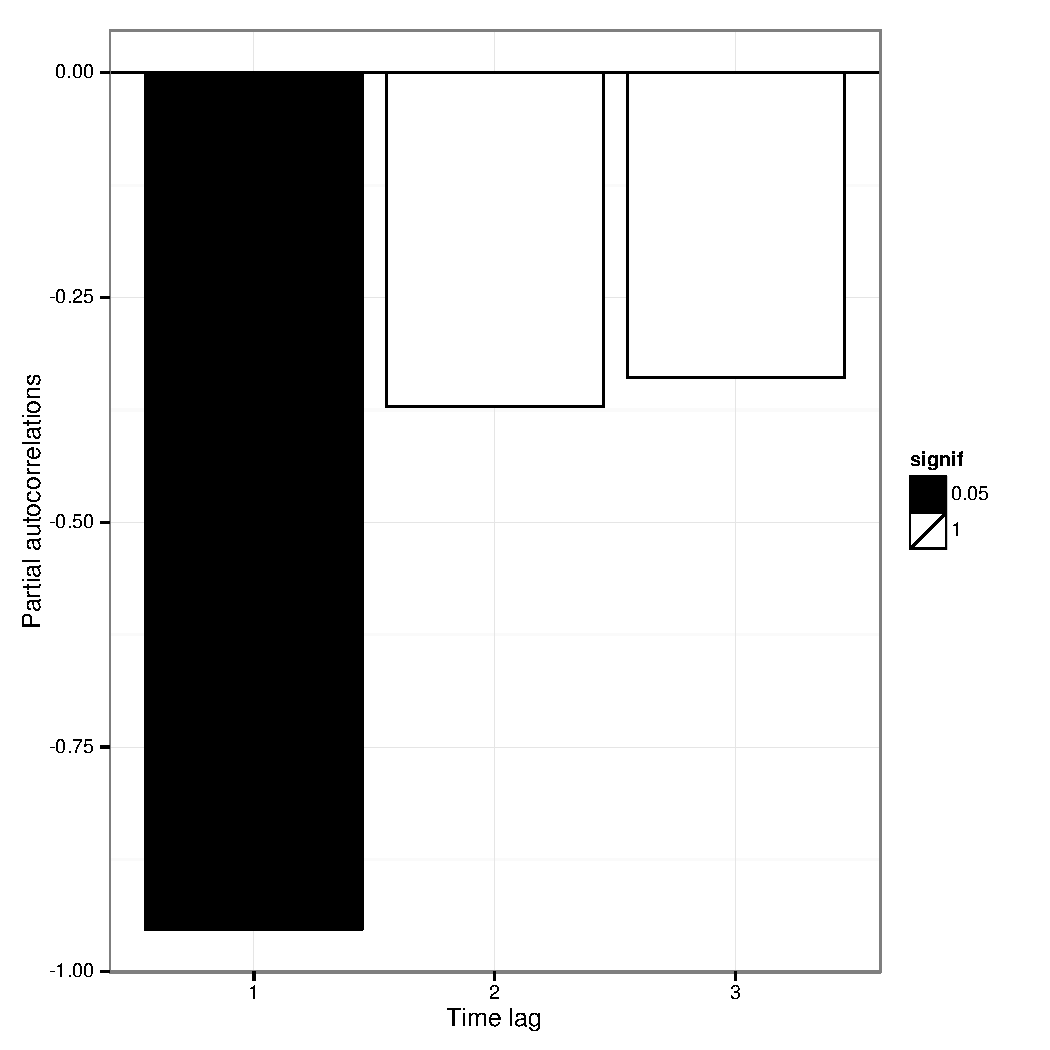
\includegraphics[width=65mm]{../White_Sea/dynamic_N_N1/perm_PRCF_Lomnishniy_detrend.pdf}
	\end{center}
	\end{minipage}

	\begin{minipage}[b]{.46\linewidth}
%Фигурка в первом ряду слева размер отведенный под весь этот объект \textendash 0.46 от ширины строки
%Параметр [b] означает, что выравнивание этих министраниц будет по нижнему краю
	\begin{center}
	{\footnotesize Южная губа о.~Ряшкова}
	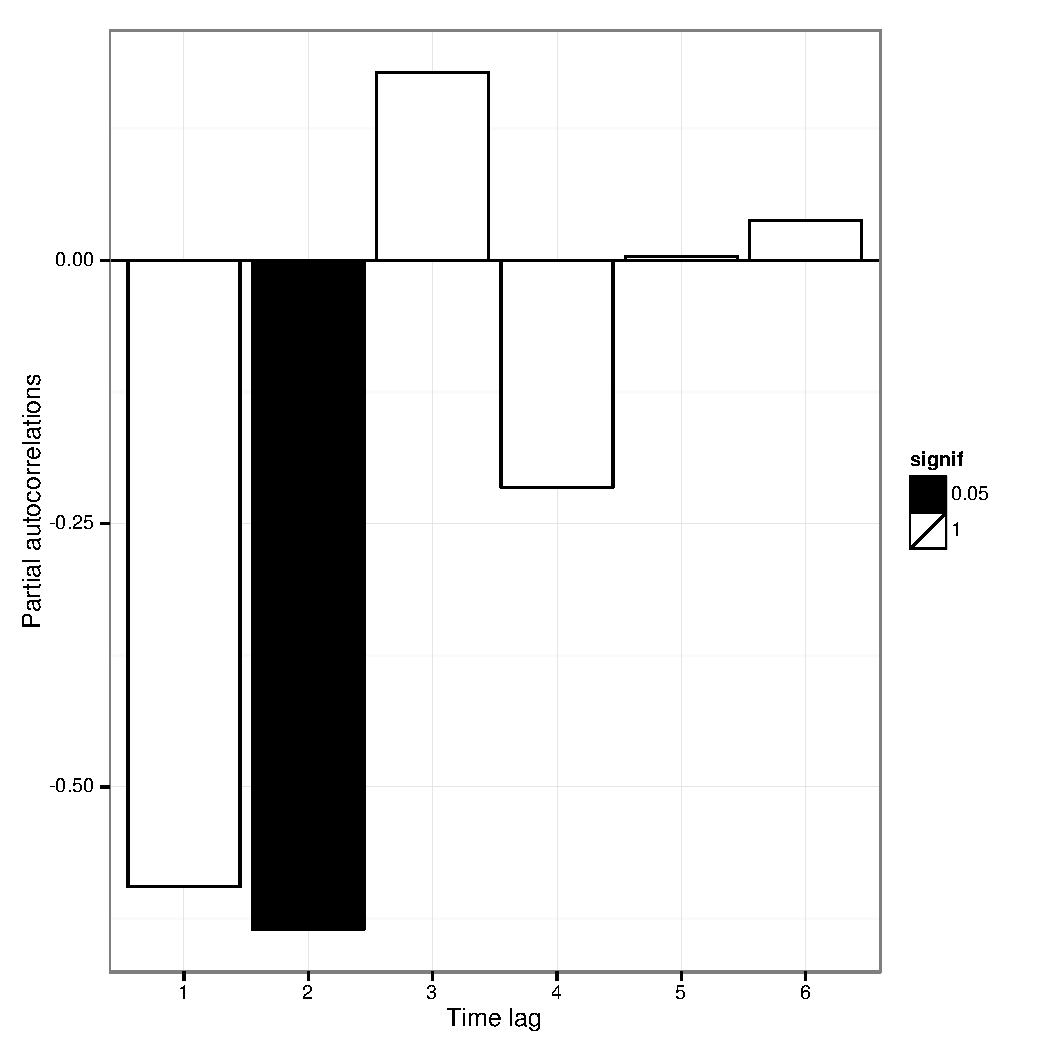
\includegraphics[width=65mm]{../White_Sea/dynamic_N_N1/perm_PRCF_YuG_detrend.pdf}
	\end{center}
	\end{minipage}
		\hfil %Это пружинка отодвигающая рисунки друг от друга
	\begin{minipage}[b]{.46\linewidth}
	\begin{center}	
	{\footnotesize Западная Ряшкова салма}
	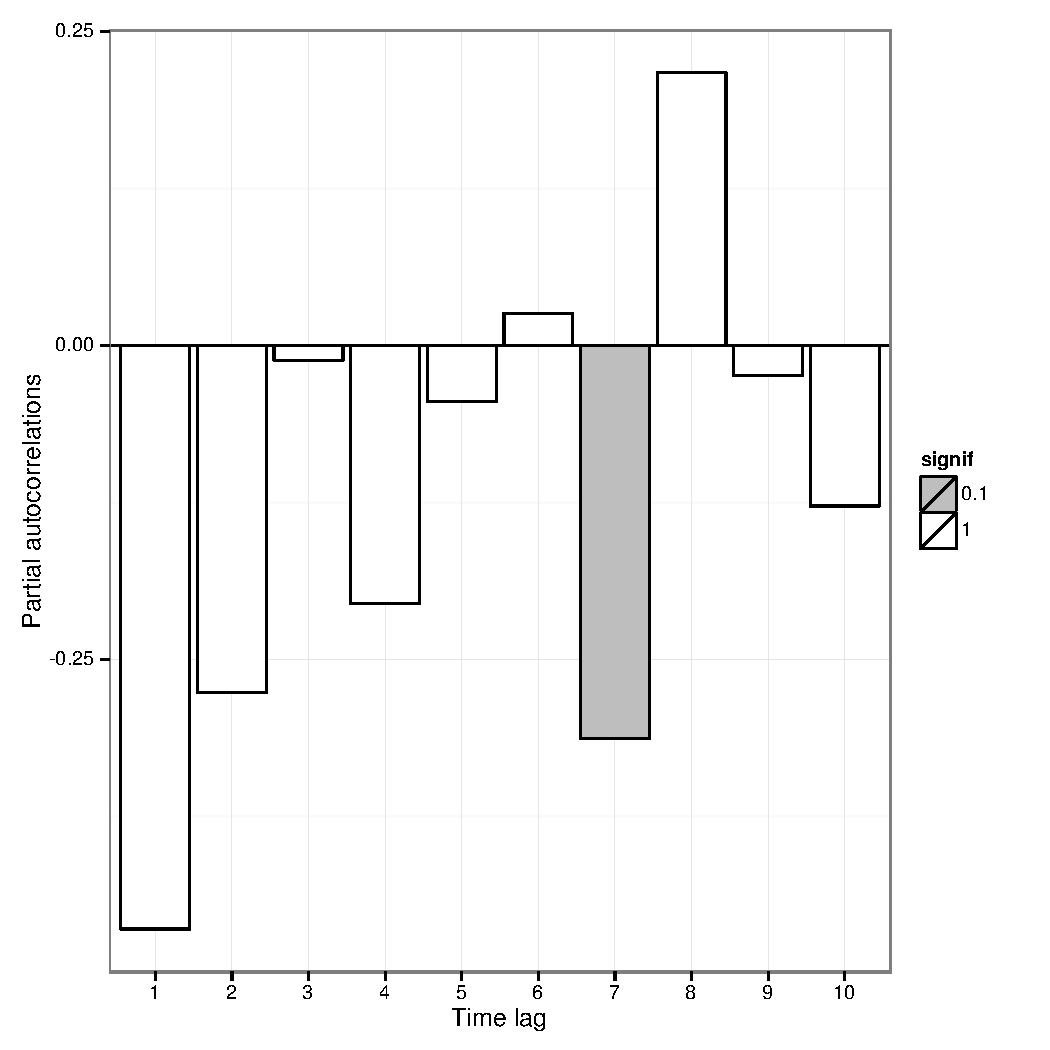
\includegraphics[width=65mm]{../White_Sea/dynamic_N_N1/perm_PRCF_ZRS_detrend.pdf}
	\end{center}
	\end{minipage}
	\caption{Частные корреляции численности {\it Macoma balthica} (без учета особей длиной менее 1 мм) в Кандалакшском заливе. Детрендированные данные. Оценка достоверности пермутационным методом.}
	\label{ris:perm_PRCF_Kandalaksha_N2_detrend}	
	\end{figure}

	\begin{figure}[ht]
%\smallskip

	\begin{minipage}[b]{.46\linewidth}
%Фигурка в первом ряду слева размер отведенный под весь этот объект \textendash 0.46 от ширины строки
%Параметр [b] означает, что выравнивание этих министраниц будет по нижнему краю
	\begin{center}
	{\tiny Медвежья}
	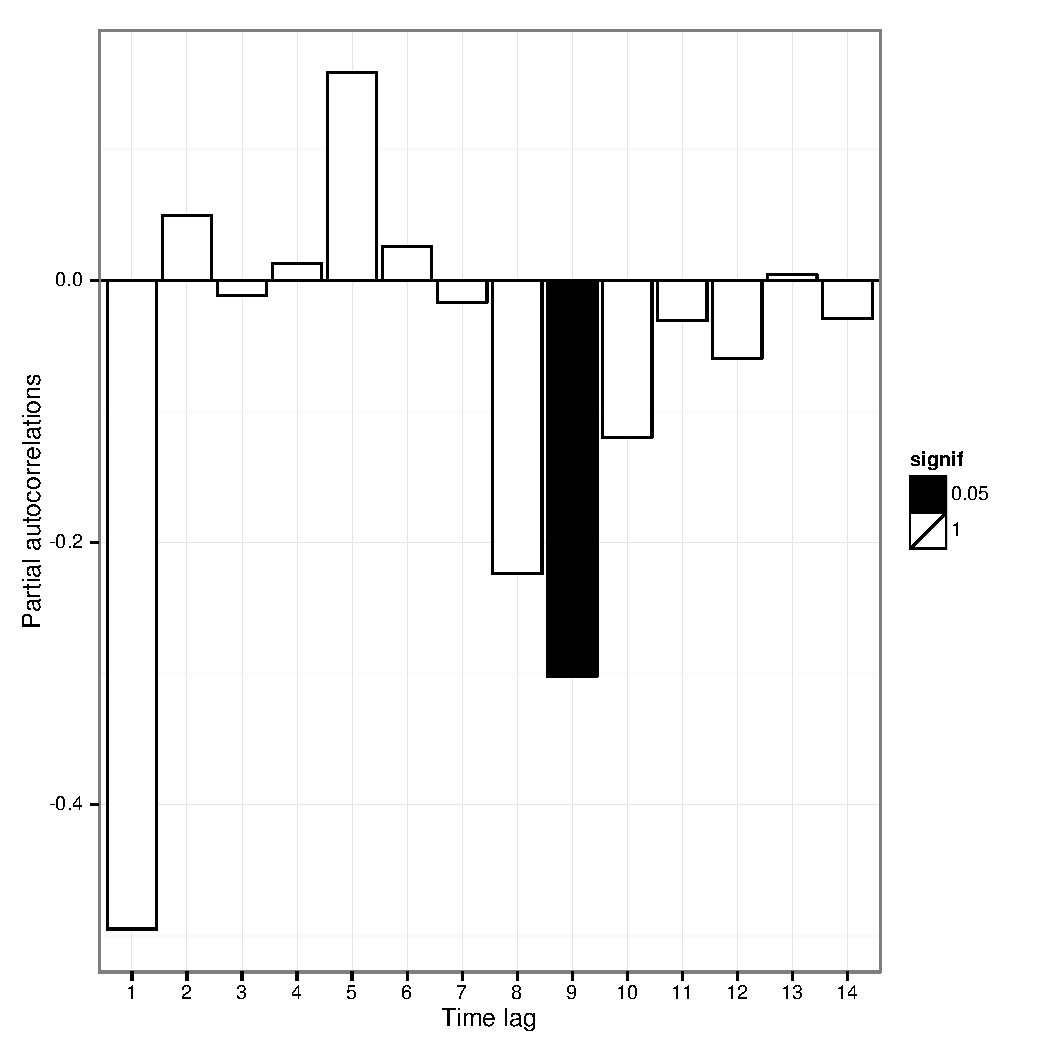
\includegraphics[width=65mm]{../White_Sea/dynamic_N_N1/perm_PRCF_Medvezhya_detrend.pdf}
	\end{center}
	\end{minipage}
%
	\hfil %Это пружинка отодвигающая рисунки друг от друга
%
	\begin{minipage}[b]{.46\linewidth}
	\begin{center}
	{\tiny Сельдяная}
	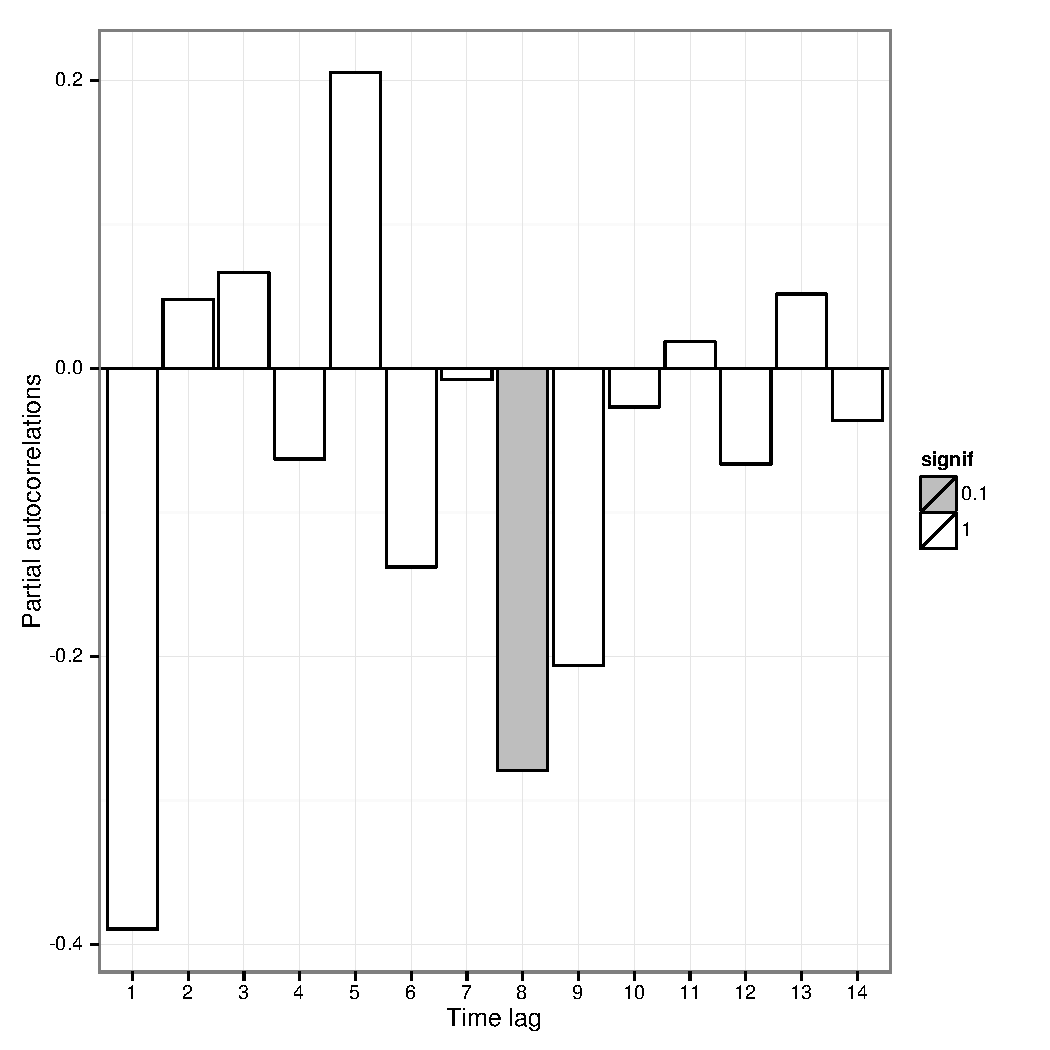
\includegraphics[width=65mm]{../White_Sea/dynamic_N_N1/perm_PRCF_Seldyanaya_detrend.pdf}
	\end{center}
	\end{minipage}

%\smallskip
%	\caption{Динамика плотности поселений {\it Macoma balthica} в вершине Кандалакшского залива}
%	\label{ris:dynamic_Kandalaksha_all}
\begin{center}
Рисунок \ref{ris:perm_PRCF_Kandalaksha_N2_detrend}, продолжение. Частные автокорреляции численности {\it Macoma balthica} (без учета особей длиной менее 1 мм) в Кандалакшском заливе. Детреднированные данные. Оценка достоверности пермутационным методом.
\end{center}
	\end{figure}
Для большинства временных рядов значение максимального значения достигает $PRCF$ с лагом 1, что характерно для динамики в отсутствие тренда. 
Достоверность частных автокорреляций оценивалась пермутационным методом.
Для участков в Южной губе о.~Ряшкова и на материковой литорали в Лувеньге были показаны достоверные значений $PRCF[2]$, причем в Южной губе $PRCF[2] > PRCF[1]$. 
Это показывает наличие в поселении плотностнозависимых процессов второго порядка.
Предположительно, это может быть воздействие хищников.
Мы надеемся проверить эту гипотезу в ходе дальнейших наблюдений.
Биологическая интерпретация $PRCF$ с большим лагом на настоящий момент представляется нам сомнительной.

		\subsection{Синхронность динамики численности {\it Macoma balthica} в Кандалакшском заливе Белого моря}
Для изучения синхронности колебаний численности маком мы использовали тест Мантеля.
Для включения большего количества рядов в анализ, он был проведен по двум наборам данных.
Первый набор данных включал участки, где при отборе проб промывка была на сите с диаметром ячеи $0,5$~мм. 
Сюда вошли участки в эстуарии р.~Лувеньги, на материковой литорали в районе Лувеньги, на о.~Горелый, в Западной Ряшковой салме и в губах Медвежья и Сельдяная.
Результаты корреляционного анализа представлены в таблице \ref{tab:Mantel_dynamic_N}.
	\begin{table}[ht]
	\caption{Синхронность динамики численности {\it Macoma balthica}.}
	\label{tab:Mantel_dynamic_N}
        \begin{tabular}{|p{0.2\textwidth}|*{8}{p{0.08\textwidth}|}} \hline
	$Mantel r \setminus p_{perm}$ & [1] & [2] & [3] & [4] & [5] & [6] & [7] & [8]
    \\ \hline
	[1] эстуарий р.~Лувеньги & & \cellcolor{yellow}{$0,002$} & $0,989$ & \cellcolor{yellow}{$0,009$} & \cellcolor{yellow}{$0,001$} & $0,264$ & \cellcolor{yellow}{$0,018$} & $0,441$
	\\ \hline
	[2] о.~Горелый & \cellcolor{yellow}{$0,929$} & & $0,393$ & \cellcolor{yellow}{$0,014$} & \cellcolor{yellow}{$0,001$} & $0,388$ & $0,992$ & $0,089$
	\\ \hline
	[3] о.~Ломнишный & $-0,439$ & $-0,067$ & & $0,208$ & $NA$ & $0,79$ & $0,082$ & $0,399$
	\\ \hline
 	[4] г.~Медвежья & \cellcolor{yellow}{$0,821$} & \cellcolor{yellow}{$0,86$} & $-0,028$ & & \cellcolor{yellow}{$0,001$} & $0,184$ & $0,932$ & $0,441$
	\\ \hline
	[5] материковая литораль (Лувеньга) & \cellcolor{yellow}{$0,781$} & \cellcolor{yellow}{$0,784$} & $NA$ & \cellcolor{yellow}{$0,704$} & & \cellcolor{yellow}{$0,044$} & $NA$ & $0,123$
	\\ \hline
	[6] г.~Сельдяная & $0,089$ & $-0,009$ & $-0,303$ & $0,087$ & \cellcolor{yellow}{$0,364$} & & $0,763$ & $0,818$
	\\ \hline
	[7] Южная губа о.~Ряшкова & \cellcolor{yellow}{$0,427$} & $-0,309$ & $0,333$ & $-0,213$ & $NA$ & $-0,127$ & & $0,585$
	\\ \hline
	[7] Западная Ряшкова салма & $-0,045$ & $0,057$ & $0$ & $-0,05$ & $0,284$ & $-0,141$ & $-0,038$
	\\ \hline
	\end{tabular}
	   {\footnotesize Примечание: Нижняя половина таблицы --- значение теста Мантеля, верхняя половина --- уровень значимости, определенный пермутационным методом. \\
Желтым выделены значения с уровнем значимости $< 0,1$. \\
$NA$ --- ряды не пересекаются во времени.}
	\end{table}
Три участка в районе Лувеньгских шхер (эстуарий р.~Лувеньги, о.~Горелый, материковая литораль) демонстрировали синхронную динамику поселений.
С данными участками была синхронна динамика поселения маком в г.~Медвежья. 
Низкая, хотя и достоверная корреляция была показана между динамикой на материковой литорали в районе Лувеньги и в г.~Сельдяной ($0,36$) и между эстуарием р.~Лувеньги и Южной губой о.~Ряшкова ($0,43$).


Второй набор данных включал участки, где при отборе проб промывку проводили на сите с диаметром ячеи $1$~мм.
Также сюда вошли те участки из предыдущего набора данных, где была известна размерная структура моллюсков --- из общей численности были вычтены численность особей длиной менее $1$~мм для возмодности сравнения.
Всего в данный анализ вошло 8 рядов данных: эстуарий р.~Лувеньги, материковая литораль в районе Лувеньги, о.~Горелый, Западная Ряшкова салма, Южная губа о.~ Ряшкова, о.~Ломнишный, б.~Клющиха и Сухая салма (табл.~\ref{tab:Mantel_dynamic_N2}).
	\begin{table}[ht]
	\caption{Синхронность динамики численности {\it Macoma balthica}.}
	\label{tab:Mantel_dynamic_N2}
        \begin{tabular}{|p{0.2\textwidth}|*{8}{p{0.08\textwidth}|}} \hline
	$Mantel r \setminus p_{perm}$ & [1] & [2] & [3] & [4] & [5] & [6] & [7] & [8]
	\\ \hline
	[1] эстуарий р.~Лувеньги & & $0,082$ & $0,646$ & $0,995$ & \cellcolor{yellow}{$0,029$} & $0,482$ & \cellcolor{yellow}{$0,013$} & $0,19$
	\\ \hline
	[2] о.~Горелый & $0,176$ &  & $0,067$ & $0,73$ & \cellcolor{yellow}{$0,001$} & $0,261$ & $0,986$ & \cellcolor{yellow}{$0,001$}
	\\ \hline
	[3] б.~Клющиха & $-0,046$ & $0,52$ &  & $0,673$ & \cellcolor{yellow}{$0,034$} & $0,213$ & $0,062$ & $0,065$
	\\ \hline
	[4] о.~Ломнишный & $-0,451$ & $-0,181$ & $-0,22$ &  & $NA$ & $1$ & $0,088$ & $0,341$
	\\ \hline
	[5] материковая литораль (Лувеньга) & \cellcolor{yellow}{$0,32$} & \cellcolor{yellow}{$0,862$} & \cellcolor{yellow}{$0,577$} & $NA$ &  & $0,117$ & $NA$ & \cellcolor{yellow}{$0,006$}
	\\ \hline
	[6]Сухая салма & $-0,019$ & $0,067$ & $0,085$ & $-1$ & $0,443$ &  & $0,688$ & $0,314$
	\\ \hline
	[7] Южная губа о.~ Ряшкова & \cellcolor{yellow}{$0,419$} & $-0,332$ & $0,434$ & $0,333$ & $NA$ & $-0,243$ &  & $0,605$
	\\ \hline
	[8] Западная Ряшкова салма & $0,114$ & \cellcolor{yellow}{$0,86$} & $0,72$ & $0,093$ & \cellcolor{yellow}{$0,755$} & $0,088$ & $-0,048$ & 
	\\ \hline
	\end{tabular}
	   {\footnotesize Примечание: Нижняя половина таблицы --- значение теста Мантеля, верхняя половина --- уровень значимости, определенный пермутационным методом. \\
Желтым выделены значения с уровнем значимости $< 0,05$. \\
$NA$ --- ряды не пересекаются во времени.}
	\end{table}
Интересно отметить, что при редукции данных до численности особей длиной более $1$~мм картина меняется.
Без изменения остается синхронность динамик поселений маком на материковой литорали в Лувеньге c о.~Горелый и эстуарием р.~Лувеньги.
Такжесохранияется синхронность динамик численности в поселениях в эстуарии р.~Лувеньга и Южной губе о.~Ряшкова.
В то же время поселение в Западной Ряшковой салме, который в предыдущем анализе показывало асинхронность по сравнению с остальными участками, в данном случае демонстрирует синхронность с поселениями на о.~Горелый и материковой литорали в Лувеньге.
Также показана синхронность динамик поселений на материковой литорали в Лувеньге и в бухте Клющиха.

Мы использовали значение теста Мантеля как меру сходства рядов данных для тестирования гипотезы, что на более близкорасположенных участках динамика численности {\it Macoma balthica} более сходна.
Для этого по координатам участков была рассчитана матрица расстояний между участками (табл.~\ref{tab:distance_area_km}).
	\begin{table}[ht]
	\caption{Расстояние между исследованными участками литорали.}
	\label{tab:distance_area_km}
        \begin{tabular}{|p{0.3\textwidth}|*{10}{p{0.04\textwidth}|}} \hline
	 & [1] & [2] & [3] & [4] & [5] & [6] & [7] & [8] & [9] & [10]
	\\ \hline
	[1] материковая литораль (Лувеньга) & 0,0 &  &  &  &  &  &  &  &  & 
	\\ \cline{1-3}
	[2] о.~Горелый & 1,5 & 0,0 &  &  &  &  &  &  &  &  
	\\ \cline{1-4}
	[3]эстуарий р.~Лувеньги & 1,0 & 1,0 & 0,0 &  &  &  &  &  &  &  
	\\ \cline{1-5}
	[4] Южная губа о.~Ряшкова & 11,7 & 10,7 & 11,7 & 0,0 &  &  &  &  &  & 
	\\ \cline{1-6}
	[5] о.~Ломнишный & 13,5 & 12,9 & 13,8 & 3,7 & 0,0 &  &  &  &  &  
	\\ \cline{1-7}
	[6] Западная Ряшкова салма & 11,9 & 10,8 & 11,8 & 1,7 & 5,3 & 0,0 &  &  &  &  
	\\ \cline{1-8}
	[7] г.~Сельдяная & 93,6 & 94,0 & 94,5 & 87,8 & 84,1 & 89,3 & 0,0 &  &  &  
	\\ \cline{1-9}
	[8] г.~Медвежья & 91,9 & 92,4 & 92,8 & 86,1 & 82,4 & 87,6 & 1,7 & 0,0 &  &  
	\\ \cline{1-10}
	[9] Сухая салма & 97,1 & 97,5 & 97,9 & 91,2 & 87,6 & 92,7 & 3,5 & 5,1 & 0,0 &  
	\\ \hline
	[10] б.~Клющиха & 100,1 & 100,6 & 101,0 & 94,8 & 91,1 & 96,3 & 8,1 & 9,7 & 5,8 & 0,0
	\\ \hline
	\end{tabular}
	   {\footnotesize Примечание:Расстояние дано в километрах.}
	\end{table}

Для обоих наборов данных тест Мантеля показал отсутсвие зависимости сходства динамики численности маком от расстояния ( $Mantel r = --0,058 (p_{perm} = 0,746)$ и $Mantel r = -0,105 (p_{perm} = 0,638)$ для первого и второго набора данных, соответственно).





		\subsection{Дальний пляж губы Дальнезеленецкая}
На данном участке использовали для промывки сито с диаметром ячеи $1$~мм и особи длиной менее $1$~мм в пробах отмечены не были. 
В течении всего периода времени плотность поселения {\it Macoma balthica} не превышала $100$~экз./м$^2$ (\ref{ris:dynamic_Zelency}). 
	\begin{figure}[h]
		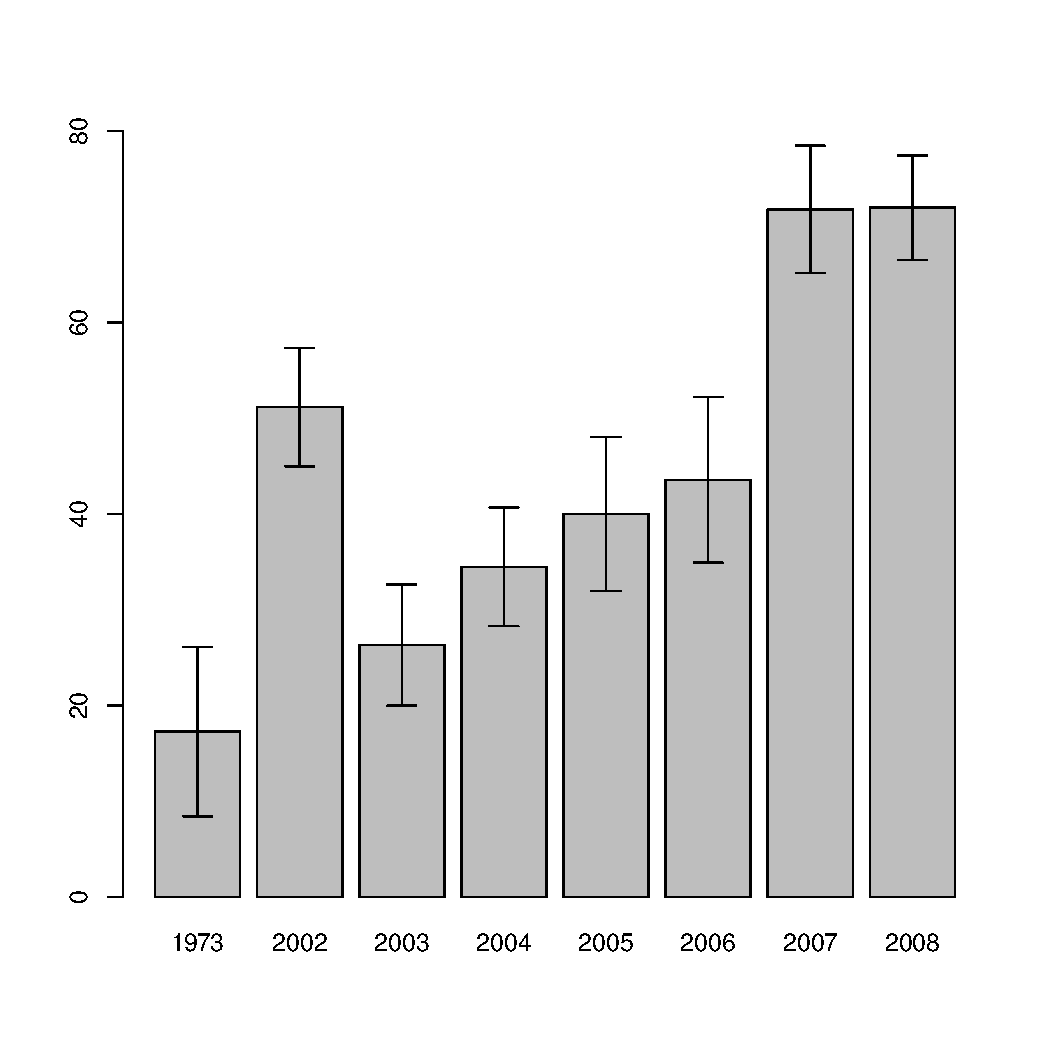
\includegraphics{../Barenc_Sea/Dalnezeleneckaya/N_dynamic_with_Agarova.pdf}
	\caption{Динамика плотности поселений {\it Macoma balthica} на литорали Дальнего пляжа г.~Дальнезеленецкой (Баренцево море)}
{\footnotesize Примечание: по оси $X$ --- годы наблюдений, по оси $Y$ --- средняя плотность поселения,~экз./м$^2$. Данные $1973$ года взяты из статьи \ref{Agarova_et_al_1976}}
	\label{ris:dynamic_Zelency}
	\end{figure}
В $2003$ году произошло уменьшение обилия маком (с $52~(13)$ до $34~(20)$~экз./м$^2$, критерий Манна-Уитни  $W = 854, p-value = 0,001$), после чего численность  в $2003 - 2006$ оставалась относительно стабильной (в среднем $33~(0,8)$~экз./м$^2$, критерий Краскела-Уоллиса $Kruskal-Wallis \chi^2 = 4,03, p = 0,26$). 
В $2007$ году численность еще увеличилась относительно предыдущего периода ($W = 1155, p-value = 8,7 \times 10^{-8}$) и оставалась стабильной к $2008$ году ($W = 516,5, p-value = 0,76$) при этом достигла уровня, максимального для всего периода ($72~(0,9)$~экз./м$^2$).

В качестве точки сравнения использовали количественные данные из статьи \ref{Agarova_et_al_1976} (\ref{ris:dynamic_Zelency}). 
Плотность поселения {\it Macoma balthica} на Дальнем пляже в $1973$ году была сравнима с таковой в $2002-2006$ годах (\ref{tab:DZ_N_1973_sravnenie}).
	\begin{table}
	\begin{tabular}{|*{4}{p{0.25\textwidth}|}} \hline
	годы сравнения & $W$ & $p-value$ & достоверность различий \\ 
	\hline
	$1973 - 2002$ & $31,5$ & $0,08$ & *\\
	\hline
	$1973 - 2003$ & $80,5$ & $0,86$ & \\
	\hline
	$1973 - 2004:2006$ &  $214$ & $0,44$ & \\
	\hline
	$1973 - 2007:2008$ & $22$ $0,0048$ & ** \\
	\hline
	\end{tabular}
	{\footnotesize Примечание: $W$ - значение критерия Вилкоксона, достоверность различий *** --- $p<0,001$; ** --- $p<0,05$; * --- $p<0,1$.}
	\caption{Сравнение численности {\it Macoma balthica} на Дальнем пляже губы Дальнезеленецкой в $1973$ году и $2002-2008$.}
	\label{tab:DZ_N_1973_sravnenie}
	\end{table}





